\section{High level Architecture}
In the following section we present the high level architecture underlying our solution. Therefore, we take into account each component individually. Once introduced the architecture, we provide an overview on the main interactions taking place between the introduced components.
\subsection{Main components}
\label{sec:architecture_diagram}
\begin{figure}[t]
\centering
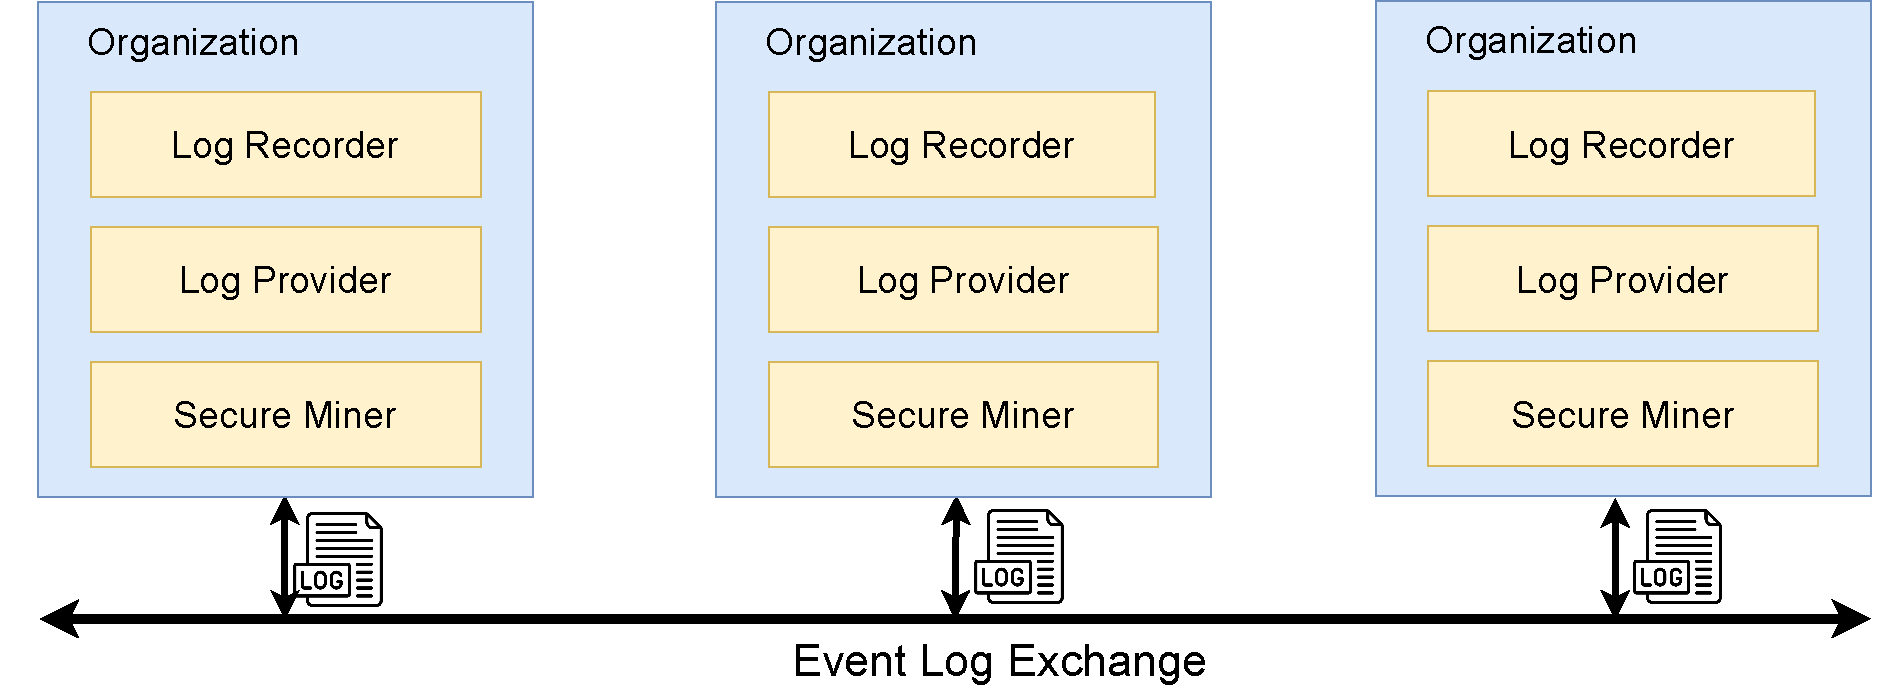
\includegraphics[width=10cm]{content/figures/architecture_diagram.pdf}
\caption{High-level architectural overview of the framework.}
\label{fig:implementation}
\end{figure}
Our architecture involve networks of nodes controlled by different \texttt{Organization}s. \texttt{Organization}s in the same network collaborate to reach a common objective sharing one or more business processes. The Hospital and Specialized Clinic, mentioned in the running examples, provide two examples of colloborative organizations. In \ref{fig:architecture_diagram}, we propose an high level schematization of our solution.
\subsubsection{ERP Interface}
\subsubsection{Log Provider}
\subsubsection{Trusted Miner}
\subsection{Workflow}
\subsubsection{Initialization}
\subsubsection{Data Exchange}
\subsubsection{Data Elaboration}



